\appendix
\section{Data Object Storage}

In the section ~\ref{sec:architecture} we supposed that all student's solutions, papers, assignments and so on are stored locally on the educator's servers. But it should be possible to introduce the new entity called "Data Object Storage" to our model(fig. ~\ref{fig:entities}). This entity should support a distributed access to all student's works. The main purposes of the data object storage are:
\begin{itemize}
\item to make publications more accessible for everyone.
\item to get rid educators of the need to store a lot of information locally without loss of security.
\end{itemize}

\begin{figure}[ht]
\centering
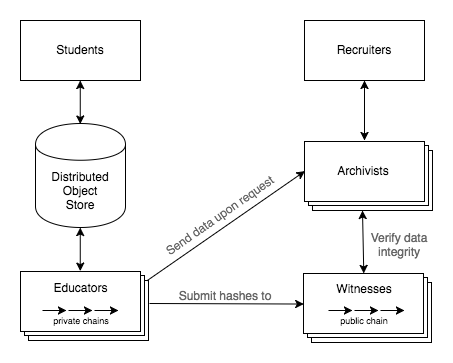
\includegraphics[width=0.8\textwidth]{entities}
\caption{Key entities of the Disciplina platform}
\label{fig:entities}
\end{figure}
